\subsection{Beschreibung der Komponenten}
\subsubsection{Rampen}
Rampen stellen Ein- und Ausgänge, sowie Zwischenlager im physischen System dar. Auf einer Rampe finden bis zu vier Pakete Platz. Bolzen hinter dem ersten Paket, separiert dieses von den anderen Dreien. Damit das vorderste Paket nicht vorne von der Rampe herunterfällt, sind an der Vorderseite zwei weitere Bolzen angebracht. Alle vier Bolzen sind seitlich der Rampe befestigt. Eine autonome Steuerung der Rampen, wird durch ein angebrachtes MICAz-Modul ermöglicht. Durch vier Lichtschranken, wird eine Überwachung der Rampe ermöglicht. Diese beinhaltet zum einen das Abfragen, wie viele Pakete auf einer Rampe liegen. Zum anderen kann durch die Überwachung überprüft werden, an welcher Stelle Pakete liegen. \autoref{fig:skiram} zeigt ein Beispiel solch einer Rampe.

\begin{figure}[h!]
	\centering
		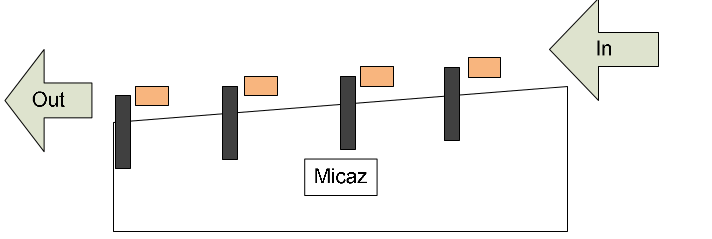
\includegraphics[width=0.9\textwidth]{SkizzeRampe.png}
	\caption{Beispiel einer eingesetzten Rampe}
	\label{fig:skiram}
\end{figure}

\subsubsection{Mikrocontroller}
Durch einen Mikrocontroller (MC) wird im Prinzip ein Mikrocomputer auf einem Chip dargestellt. Solch ein Mikrocomputer ist ein Rechner, dessen Zentraleinheit aus einem oder mehreren Mikroprozessen besteht. Zusätzlich enthält ein Mikrocomputer Speicher, ein Verbindungssystem und Ein- bzw. Ausgabeschnittstellen. Das Ziel eines Mikrocontroller ist es, eine Kommunikations- oder Steuerungsaufgabe mit möglichst wenig Bauteilen zu lösen. Der in einem Mikrocontroller verbaute Prozessorkern, Speicher und die Aus- und Eingabeschnittstellen eines Mikrocontroller, sind auf die Lösung solcher Aufgaben zugeschnitten. Die große Anzahl an potenzieller Aufgabenstellung hat zur Folge, dass es eine Vielfalt von Mikrocontrollern gibt. Meist sind die Mikrocontroller deshalb in Mikrocontrollerfamilien aufgeteilt. Innerhalb einer Familie unterscheiden sich die Controller nicht im Prozessorkern, sondern im Speicher und in den Ein- und Ausgabeschnittstellen \cite{ECHT2005}. In \autoref{fig:aufbmc} ist der schematische Aufbau eines solchen Controllers dargestellt.
\begin{figure}[th]
	\centering
		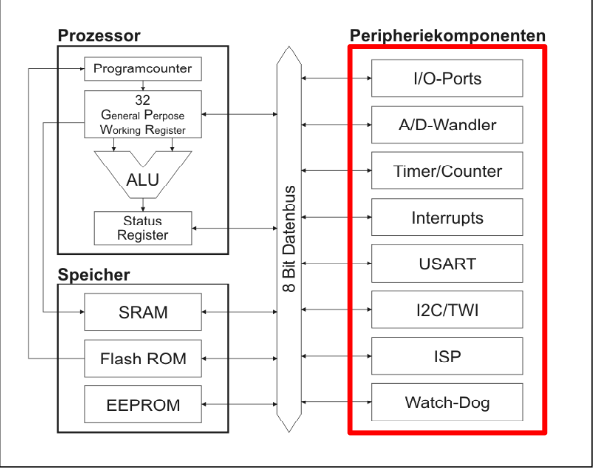
\includegraphics[width=0.9\textwidth]{Aubau_eines_Mikrocontrollers.png}
	\caption{Schematischer Aufbau eines Mikrocontrollers \cite{habil:Ostermeye:2014:Online}}
	\label{fig:aufbmc}
\end{figure}

\begin{itemize}
\item Prozessor (CPU)
\begin{itemize}
          \item Arithmetic Logic Unit, kurz ALU (Rechenwerk)
          \item 32 GPIO-Register (Arbeitsregister für ALU)
          \item Programmcounter (Programmposition)
					\item Statusregister (Status der aktuellen Operation) 
\end{itemize}
\item Speicher
\begin{itemize}
          \item SRAM Datenspeicher (Static Random-Access Memory)
					\item Flash ROM Programmspeicher (Read Only Memory)
					\item EEPROM Festspeicher (Electrically Erasable Programmable Read-Only Memory)
\end{itemize}
\item Peripheriekomponenten
    \begin{itemize}
          \item I/O-Ports Primärfunktion der Pins (Ein- und Ausgänge)
          \item A/D-Wandler (Einlesen von analogen Spannungen)
          \item Timer/Counter (Zeitintervall-/PBM-Generator)
					\item Interrupts (Programmunterbrechungsroutinen)
					\item USART, I2C/TWI und SPI (Kommunikationsschnittstellen)
					\item Watch-Dog (Absicherung gegen Systemfehler)
					\item ISP (Schnittstelle zum \"{U}bertragen des kompilierten Programms)
	\end{itemize}
\end{itemize}
Mikrocontroller sind im heutigen Leben weit verbreitet und es gibt eine große Anzahl von Herstellern, die Mikrocontroller anbieten.
Im Folgenden werden einige Hersteller mit ihren MC-Familien beispielhaft aufgeführt:
\begin{itemize}
\item Intel (8051-Serie)
\item Renesas (H8)
\item Zilog (Z8)
\item Microchip (Pic)
\item Freescale (früher Motorola) (68HC08 bzw. 68HCS08)
\item Atmel (AVR, 8051-Serie)
\end{itemize}
Für das Projekt FAISE wurde die Atmel-Serie eingesetzt. Es sind Mikrocontroller mit erweiterten Peripherien und Funktionen, 
die auf der 8-Bit-AVR-Architektur basieren. Bei AVR handelt es sich um einen RISC-Kern, der an der Universität von Trondheim 
in Norwegen entwickelt und von Atmel aufgekauft wurde. Die CPU besitzt 32 allgemeine 8-Bit Register (general purpose registers) 
und ist in der Lage in einem einzigen Taktzyklus Daten aus zwei beliebigen Registern in die ALU zu laden, diese zu verarbeiten 
und das Ergebnis in einem beliebigen Register zu speichern \cite[vgl.]{Viktor:Seib:2014:Online}. Die Konfiguration eines Atmega 8 der Firma Atmel sieht so aus:
\begin{figure}[h!]
	\centering
		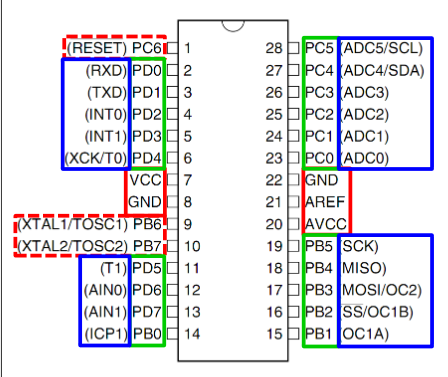
\includegraphics[width=0.9\textwidth]{Atmel8.png}
	\caption{Atmel 8 \\ \url{(http://www.ids.tu-bs.de/tl\_files/Lehre/Vorlesungen/Simulation2/Einfuehrung\_in\_die\_MC\_Programmierung\_Teil1.pdf)}}
	\label{Atmel 8}
\end{figure}
\begin{figure}[h!]
	\centering
		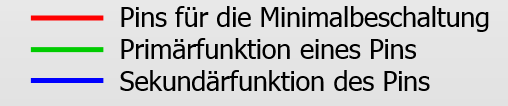
\includegraphics[width=0.9\textwidth]{LegendeAtmel8.png}
	\caption{Atmel 8 \url{(http://www.ids.tu-bs.de/tl\_files/Lehre/Vorlesungen/Simulation2/Einfuehrung\_in\_die\_MC\_Programmierung\_Teil1.pdf)}}
	\label{Legende Atmel8}
\end{figure}
\begin{itemize}
\item Pins für die Minimalbeschaltung
\begin{itemize}
          \item Spannungsversorgung
          \item Referenzspannung/Taktgeber
          \item Reset      
					\end{itemize}
\item Primärfunktion eines Pins
\begin{itemize}
          \item Ein- bzw. Ausgang
					\end{itemize}
\item Sekundärfunktion des Pins
\begin{itemize}
          \item A/D-Wandlereingang
          \item Ext. Interrupt
          \item PBM-Ausgang   
\end{itemize}
\end{itemize}
Für die Programmierung der AVR-Controller gibt es eine kostenlose Entwicklungsumgebung AVR-Studio, die das Einbinden des Compilers problemlos erlaubt.

\paragraph{ Sensorik und Aktorik}
Hauptziel der Teilgruppe Materialfluss ist das Management von Paketen auf einer Rampe.
Die Aufgabe der Sensorik ist dabei, dass die mit Lichtschranken ausgestatteten Rampen Pakete detektieren und auf Änderungen der Positionen der Pakete reagieren.
Die Lichtschranken bestehen aus einer Lichtstrahlenquelle (dem Sender) und einem Sensor (dem Empfänger) f\"{u}r diese Strahlung.
Als Lichtquelle kommt Infrarotlicht zum Einsatz und der Vorteil besteht in der einfachen Einstellung des Sensorsystems durch den
sichtbaren Lichtfleck. Das Funktionsprinzip der Lichtschranke besteht darin, den sich  ändernden Zustand durch die Lichtintensität mit dem Sensor zu registrieren. 
Die Rampen werden auf Hardwareebene um eine Aktorik zum Arretieren der Kisten ergänzt. Diese Aktoren (in unserem Fall die
eingesetzte Bolzenpaare) sind für das Ausführen von Bewegungen zuständig.
Sie sind aktive Stellelemente, die in der Antriebs- und Steuerungstechnik vom  Mikrorechner angesteuert werden, um das Verhalten des Prozesses durch das vom Sensor kommende Signal in einer gew\"{u}nschten Weise zu ermöglichen. In dieser allgemeinen Darstellung stehen die 
Ausgangssignale eines Sensors und die Stellsignale der Aktoren mit einem
Informationsverarbeitungssystem (IVS) in Verbindung.
